\documentclass[13pt,a4paper]{article}

\usepackage[utf8]{inputenc}
\usepackage{graphicx}
\usepackage{wrapfig}
\usepackage{color}
\usepackage{xcolor}
\usepackage{amsmath}
\usepackage{amssymb}
\usepackage[inkscapelatex=false]{svg}
\usepackage{array, makecell}
\usepackage{mhchem}
\usepackage{tabularx}
\usepackage{svg}
\usepackage{braket}
\usepackage{listings}
\definecolor{commentsColor}{rgb}{0.497495, 0.497587, 0.497464}
\definecolor{keywordsColor}{rgb}{0.000000, 0.000000, 0.635294}
\definecolor{stringColor}{rgb}{0.558215, 0.000000, 0.135316}
\lstset{
    frame=single,
    language=Python,
    basicstyle=\ttfamily\vspace{1em},
}

\usepackage[T1]{fontenc}
\usepackage[utf8]{inputenc}
\usepackage[lf]{Baskervaldx} % lining figures
\usepackage[bigdelims,vvarbb]{newtxmath} % math italic letters from nimbus Roman
\usepackage[cal=boondoxo]{mathalfa} % mathcal from STIX, unslanted a bit
\renewcommand*\oldstylenums[1]{\textosf{#1}}

\usepackage{multicol}
\usepackage{colortbl}
\usepackage[Export]{adjustbox}
\adjustboxset{max size={0.9\linewidth}{0.9\paperheight}}
\usepackage[colorlinks=true,linkcolor=red,citecolor=green]{hyperref}

\textwidth=16cm
\textheight=23cm
\topmargin=-2cm
\oddsidemargin=0cm
\setlength{\parindent}{0em}
\setlength{\parskip}{0.6em}
\setlength{\jot}{12pt}
\renewcommand{\arraystretch}{1.4}
\renewcommand{\theadfont}{\bfseries}
\newcommand{\todo}[1]{\textcolor{red}{TODO: #1}}


\begin{document}
\title{
    \LARGE
    \textbf{SATFD - lab 01 report}
}
\author{
    \large
    Dawid Karpiński, 8.03.2024 r.
}
\date{}
\maketitle

\section{Wave}

The task during lab 01 involves determining the highest peaks in the spectrum of a sound file and identifying what guitar chord has been recorded.

The available file, \verb|chord.wav|, is a recording of a guitar playing some chord. The signal is a 44100 [Hz] sample rate and was cut to 4 seconds of data.

\begin{lstlisting}[caption={\textbf{Code snippet for loading the initial signal.}}]
sample_rate, wave = scipy.io.wavfile.read("./data/chord.wav")
time = np.arange(wave.size) / sample_rate
\end{lstlisting}

\begin{figure}[ht!]
    \centering
    \caption{\textbf{Wave from 'chord.wav'.}}
    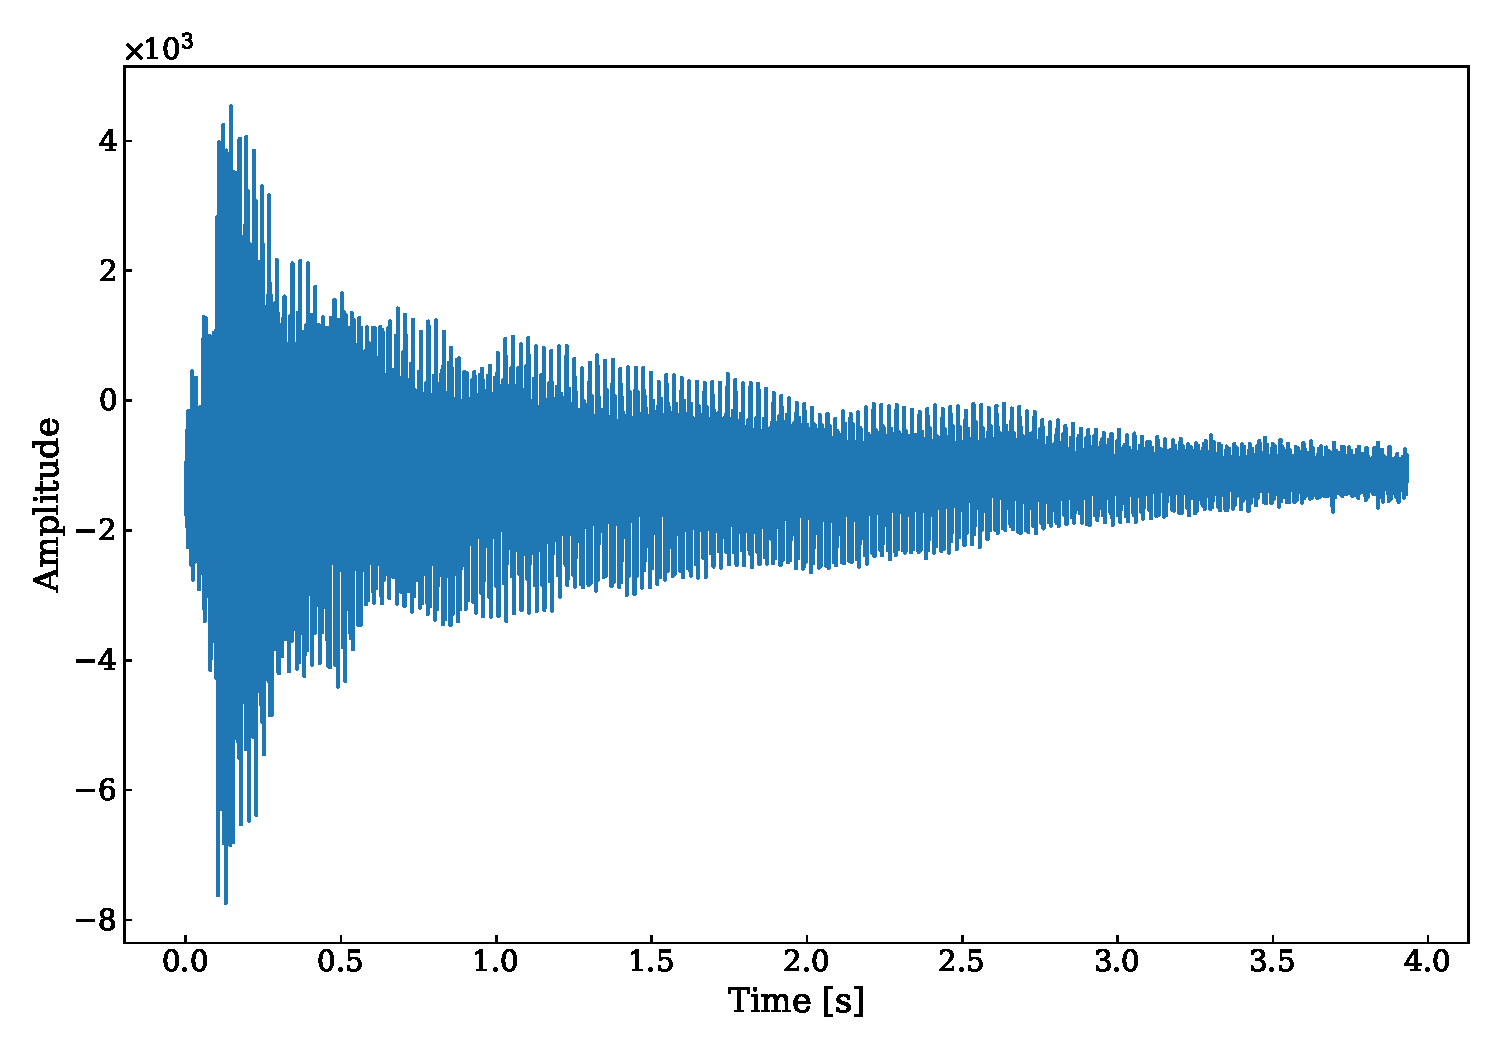
\includegraphics[width=1\textwidth]{wave.pdf}
\end{figure}

\pagebreak
\section{Fourier transform and the power spectrum}

To determine the tones in the recorded accord, a Fourier transform was performed using the function \verb|np.fft.fft()|. The power spectrum of the signal was limited to the frequency range of 16 to 4000 [Hz], as suggested in the lab instructions.

Furthermore, the power in dB units is obtained by using the following formula:
$$
P(x) = 10 \cdot \log(|H(x)|),
$$
where $H(x)$ is a Fourier transform of the initial signal

\begin{lstlisting}[caption={\textbf{Code snippet for calculating the power spectrum.}}]
spectrum = np.fft.fft(wave)
freqs = np.fft.fftfreq(wave.size, 1 / sample_rate)

f_range = (freqs >= 16) & (freqs <= 4e3)
freqs = freqs[f_range]
spectrum = spectrum[f_range]

spectrum_db = 10 * np.log10(np.abs(spectrum) + 1e-15)
\end{lstlisting}

\begin{figure}[ht!]
    \centering
    \caption{\textbf{Power spectrum of 'chord.wav'.}}
    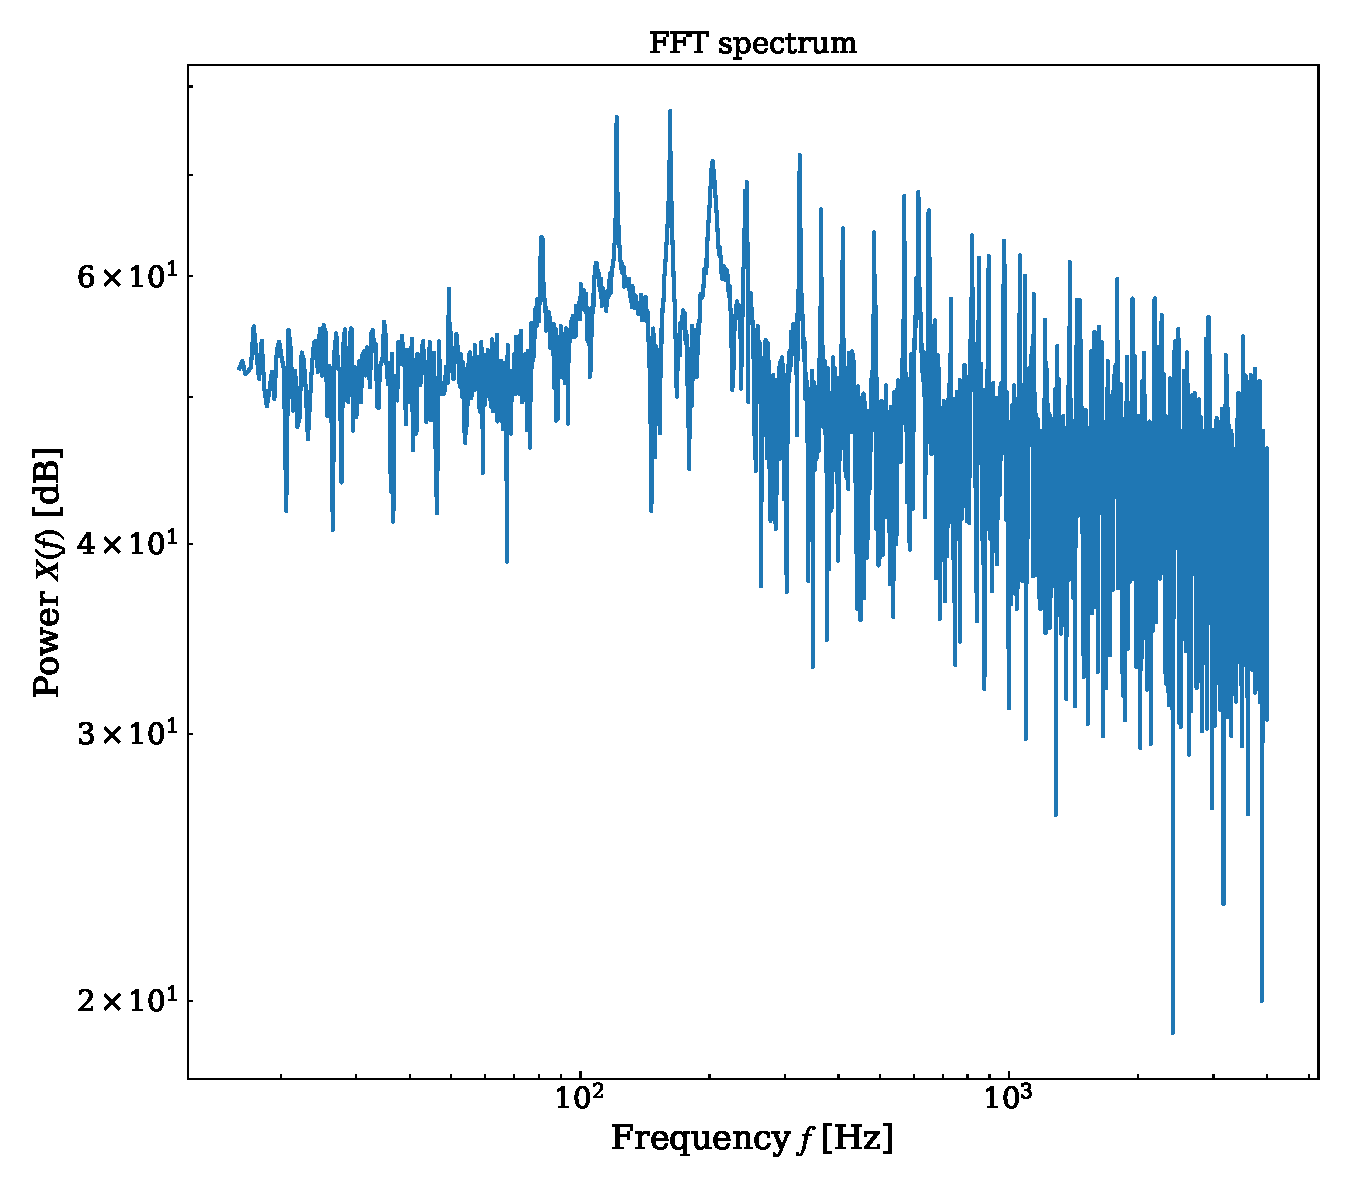
\includegraphics[width=1\textwidth]{fourier.pdf}
\end{figure}


\section{Peak analysis}
By using the \verb|scipy.signal.find_peaks()| function, the frequencies corresponding to the highest value of power are found, and only 11 highest are considered for further analysis.

\begin{lstlisting}[caption={\textbf{Code snippet for identifying the semitones, based on the provided MATLAB code.}}]
peaks, _ = signal.find_peaks(spectrum_db, distance=100)
peaks = peaks[np.argsort(spectrum_db[peaks])[-11:]]

min_note = -57
max_note = 39

base_names = ["C", ..., "B"]

tone_freqs = 440 * np.power(2, np.arange(min_note, max_note + 1) / 12)
tone_names = [
    *[
        f"{base_names[halftone]}{octave}"
        for octave in range(8)
        for halftone in range(12)
    ],
    "C8",
]
\end{lstlisting}

\begin{figure}[ht!]
    \centering
    \caption{\textbf{The highest peaks and the corresponding semitones.}}
    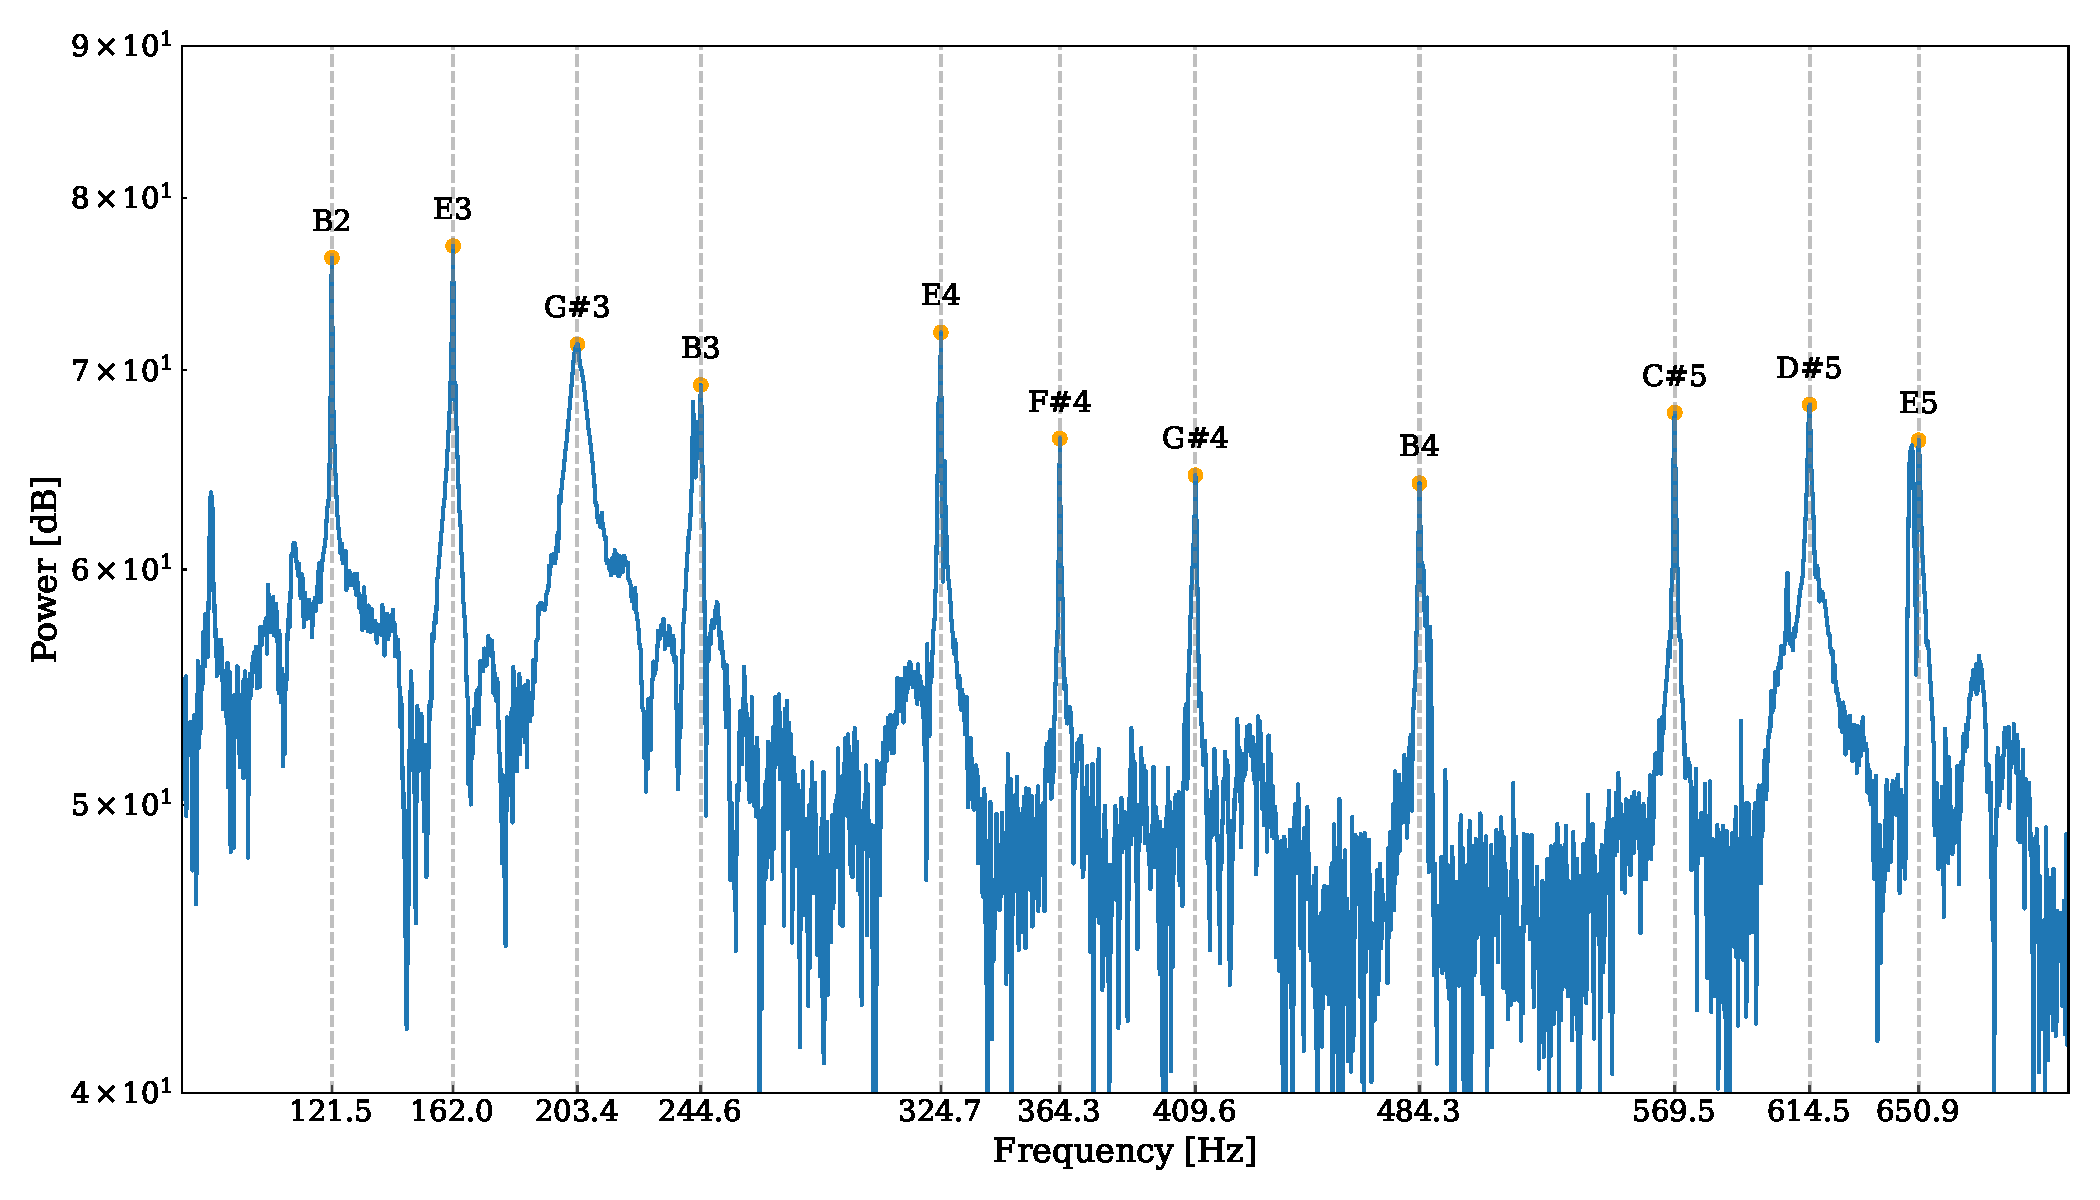
\includegraphics[width=1\textwidth]{peaks.pdf}
\end{figure}

The played chord is in the major key, hence one of the possibly played chords could be \textbf{E major}. It consists of E, G\# and B, which are showing as peaks in the above plot of the power spectrum.


\section{Conclusion}

By taking a Fourier transform and representing the signal as a power spectrum, I have identified E major as the key of the chord from the provided sound file \verb|chord.wav|.

The entire code for generating the data and plots can be found at:

\url{https://github.com/davkk/signal-analysis/tree/main/sat/lab01}

\end{document}
